\documentclass[12pt]{article} 
\usepackage[utf8]{inputenc}
\usepackage[T1]{fontenc} 
\usepackage[portuguese]{babel} 
\usepackage{graphicx}
\usepackage{hyperref} 
\usepackage{booktabs} 
\usepackage{url}
\usepackage{amsmath}
\usepackage{geometry} 
\geometry{a4paper, margin=1in}

\title{Relatório de Análise de Série Temporal no Mercado Imobiliário}
\author{Gabriel Fruet} \date{\today}

\begin{document}

\maketitle

\section{Introdução} Este relatório apresenta uma análise da série temporal da
razão de consumidores entre 38 e 58 anos em relação ao número de empresas
ativas por estado, no período de 2007 a 2022. Utilizei dados da SCOD Brasil e
do IBGE para realizar esta análise.

\section{Metodologia} 

\subsection{Coleta de Dados} Os dados das empresas foram
obtidos da Tabela 1757 do SIDRA, utilizando requisições HTTP diretamente
através da biblioteca \texttt{requests}, sem o uso de bibliotecas prontas como
\texttt{sidrapy}. 

Para obter os dados do SIDRA, utilizei a seguinte URL 
\url{https://apisidra.ibge.gov.br/values/t/1757/n2/all/p/2007-2020}.
A interpretação dessa URL é esta: Consulte no SIDRA os valores da tabela 1757,
para todos os componentes do  nível territorial n2 (Grande Região) entre os 
anos de 2007 e 2020

A população estimada foi obtida da projeção populacional
disponibilizada pelo IBGE, através da URL \url{https://ftp.ibge.gov.br/Projecao_da_Populacao/Projecao_da_Populacao_2024/projecoes_2024_tab1_idade_simples.xlsx}.

\subsection{Tendência dos dados}

\begin{figure}[!htbp]
    \begin{center}
    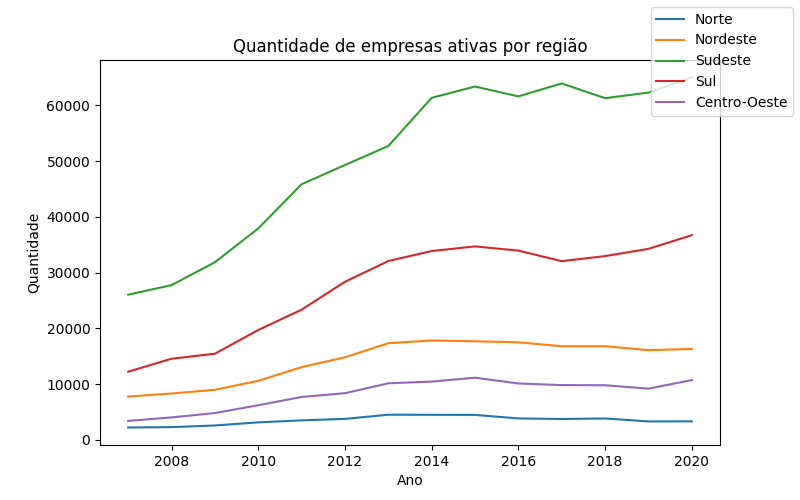
\includegraphics[width=0.7\textwidth]{../figures/time_series_business.png}
    \caption{\label{fig:trend_bus} Comportamento da quantidade de empresas ativas por ano}
    \end{center}
\end{figure}

\begin{figure}[!htbp]
    \begin{center}
    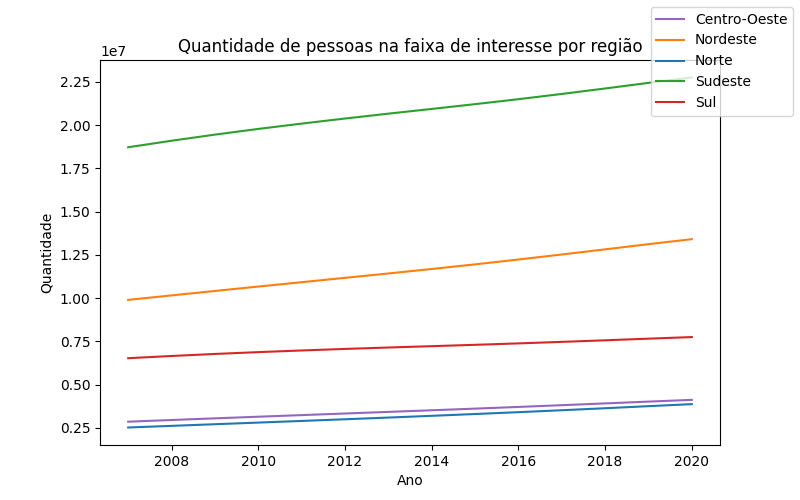
\includegraphics[width=0.7\textwidth]{../figures/time_series_population.png}
    \caption{\label{fig:trend_pop} Comportamento da população entre 38 e 58 anos por ano}
    \end{center}
\end{figure}

\begin{figure}[!htbp]
    \begin{center}
    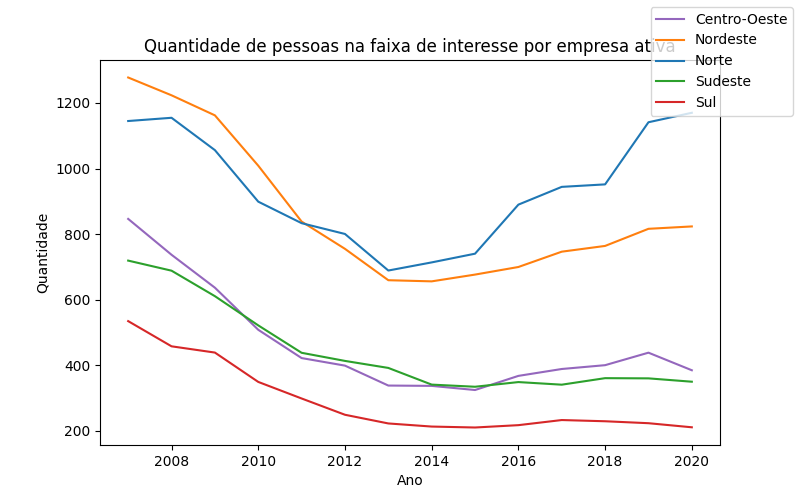
\includegraphics[width=0.7\textwidth]{../figures/time_series_ratio.png}
    \caption{\label{fig:trend_rat} Comportamento da quantidade de pessoas na faixa de interesse por empresas ativas por ano}
    \end{center}
\end{figure}

Como podemos ver na fígura \ref{fig:trend_pop}, a população vem aumentando
desde 2008. Ademais, de acordo com a fígura \ref{fig:trend_bus}, a quantidade
de empresas ativas no setor de construção também têm aumentado desde 2008,
apesar de uma leve desaceleração em torno de 2014, possivelmente devido à crise
que o país sofreu.

Ao combinar esses dados em uma razão, percebemos que através da fígura
\ref{fig:trend_rat} a tendência no período de 2014, foi uma diminuição na
demanda por empresas do ramo de construção, possivelmente devido a falência de
empresas, já que a população não costuma diminuir bruscamente. Porém, houve um aumento
e retorno significativo, especialmente após 2016 na Grande Região Norte.



\subsection{Analise de Estacionaridade} 

\begin{figure}[!htbp]
    \begin{center}
    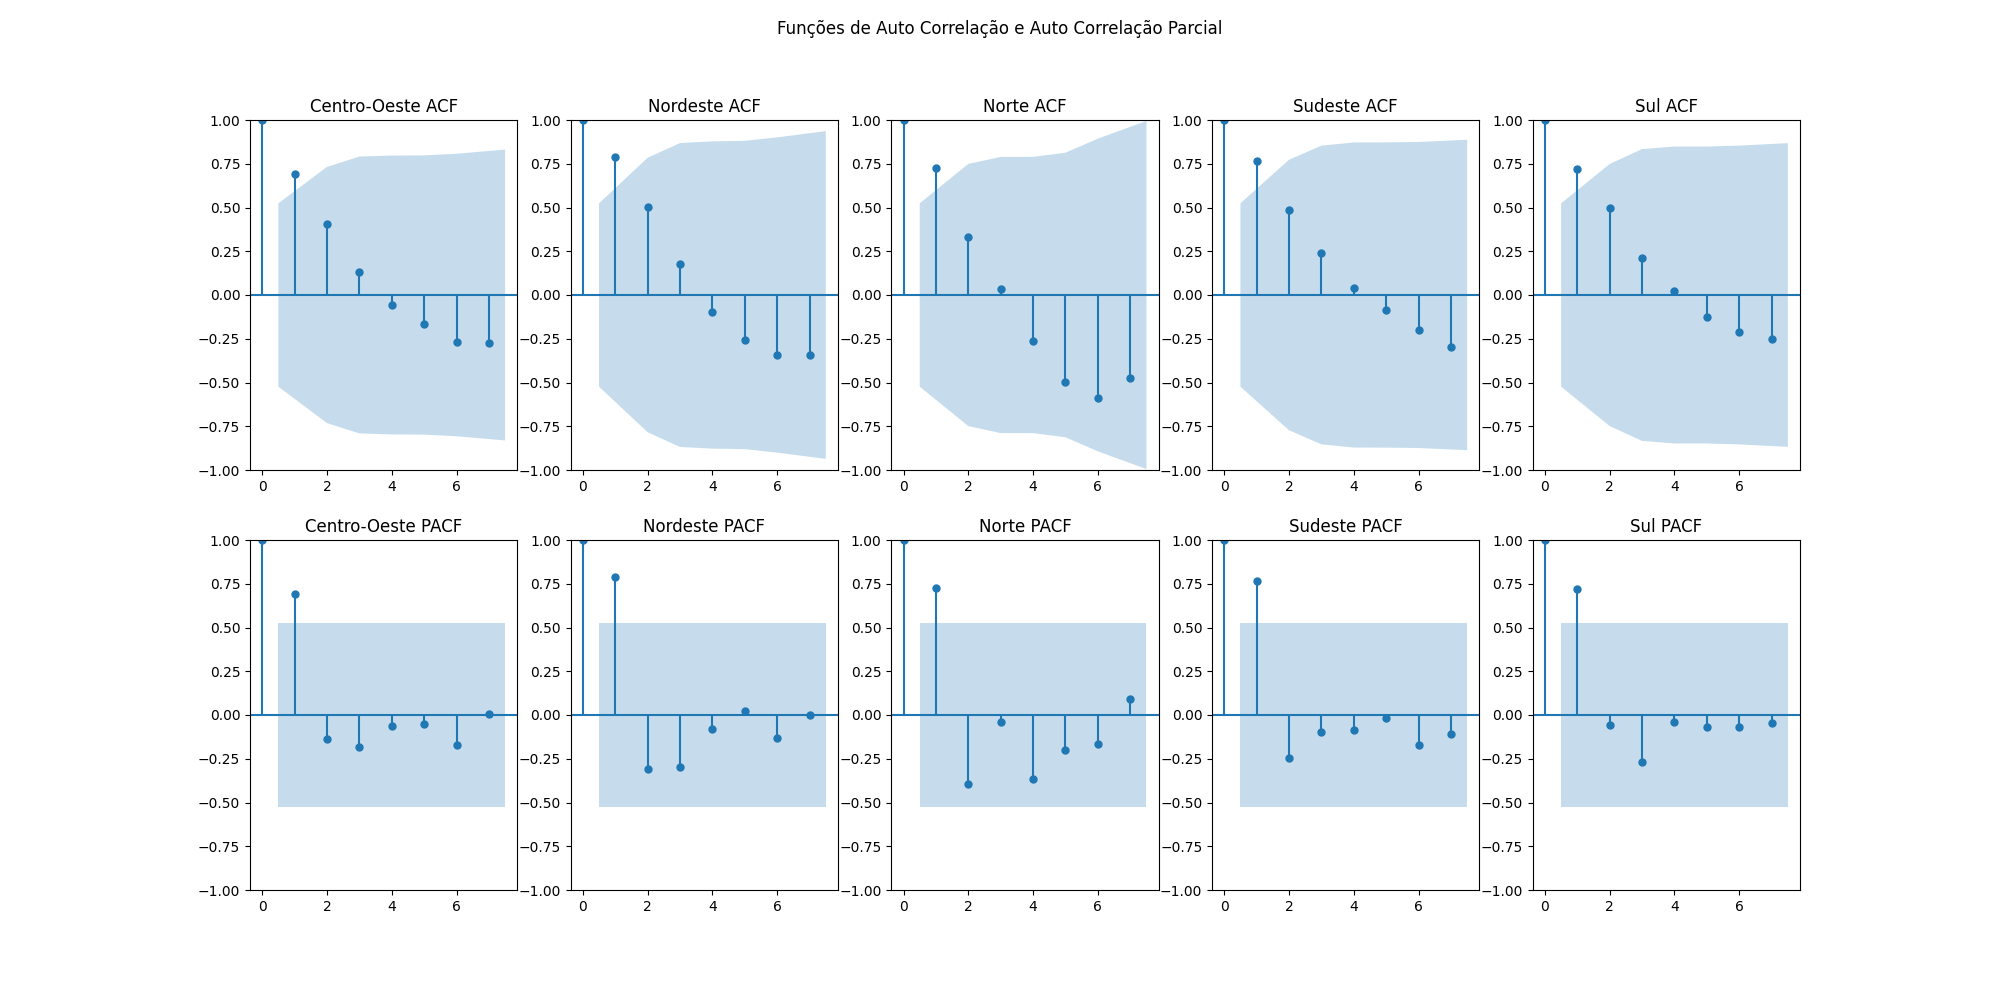
\includegraphics[width=\textwidth]{../figures/acf_pacf.png}
    \caption{\label{fig:corr} PACF e ACF para cada Grande Região do país.}
    \end{center}
\end{figure}

Quando lidamos com series temporais, uma das primeiras abordagens
é checar sua estacionaridade, para compreender quais técnicas são 
aplicáveis.

De acordo com a fígura \ref{fig:corr}, podemos perceber que a ACF 
decai gradualmente, o que indica que há algum tipo de tendência nos
dados. Além disso, a PACF só tem correlação significative com o primeiro lag,
evidenciando que somente a amostra imediatamente passada deve influenciar de
maneira consistente nossas predições. Cabe ressaltar que o ACF decai gradualmente
pois ele leva em conta as correlações acumuladas entre lags, já o PACF não. 

\subsection{Escolha do Modelo ARIMA}

\begin{table}[h!]
\centering
\caption{Melhores parâmetros de ordem ARIMA após validação cruzada}
\label{tab:arima_performance}
\begin{tabular}{lcccc}
\toprule
\textbf{Region} & \textbf{RMSE} & \textbf{AR Order} & \textbf{I Order} & \textbf{MA Order} \\
\midrule
Centro-Oeste  & 27.827 & 1 & 1 & 0 \\
Nordeste  & 23.064 & 1 & 1 & 0 \\
Norte  & 107.637 & 1 & 1 & 0 \\
Sudeste  & 12.379 & 1 & 0 & 0 \\
Sul  & 9.938 & 1 & 1 & 0 \\
\bottomrule
\end{tabular}
\end{table}

\section{Resultados} 

\subsection{Análise Temporal} Apresentamos aqui os
gráficos e tabelas que mostram a evolução da razão de consumidores por estado.

\subsection{Estados Saturados e Oportunidades} Identificamos os estados que
apresentam saturação no mercado e aqueles com maiores oportunidades futuras.

\section{Conclusão} Concluímos com as principais descobertas e recomendações
baseadas na análise dos dados.

\section*{Referências} 
\begin{itemize} 
    \item SCOD Brasil. Tendências do mercado
    imobiliário para 2023. Disponível em: \url{https://scod.com.br/blog/post/tendências-do-mercado-imobiliário-para-2023}
    \item IBGE. Tabela 1757 - Dados gerais das empresas de construção. Disponível em: \url{https://apisidra.ibge.gov.br/home/ajuda} 
    \item IBGE. Projeção da população. Disponível em: \url{https://www.ibge.gov.br/estatisticas/sociais/populacao/9109-projecao-da-populacao.html}
\end{itemize}

\end{document}
